
\subsubsection{Interaction}
\label{sec:Interaction}

The \sbol{Interaction} class (as shown in \ref{uml:interaction}) provides more detailed description of how the \sbol{Feature} objects of a \sbol{Component} are intended to work together.  
For example, this class can be used to represent different forms of genetic regulation (e.g., transcriptional activation or repression), processes from the central dogma of biology (e.g. transcription and translation), and other basic molecular interactions (e.g., non-covalent binding or enzymatic phosphorylation).
Each \sbol{Interaction} includes \sbolmult{type:I}{type} properties that refer to descriptive ontology terms and \sbol{hasParticipation} properties that describe which \sbol{Feature} objects participate in which ways in the \sbol{Interaction}.

\begin{figure}[ht]
\begin{center}
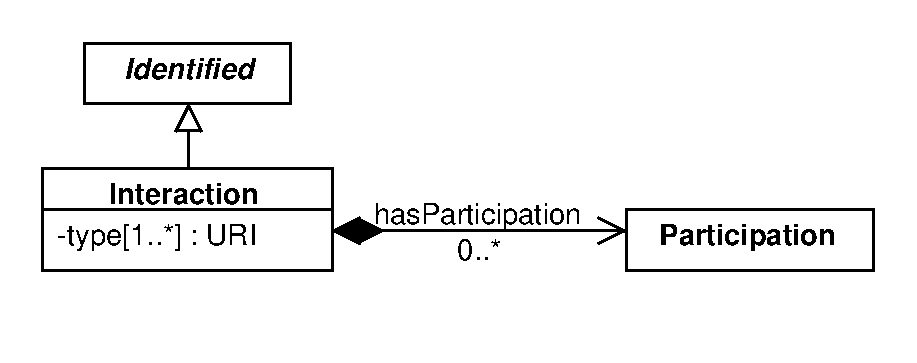
\includegraphics[scale=0.6]{uml/interaction}
\caption[]{Diagram of the \sbol{Interaction} class and its associated properties.}
\label{uml:interaction}
\end{center}
\end{figure}

\subparagraph{The \sbolheading{type} property}\label{sec:type:I}

An \sbol{Interaction} is REQUIRED to have one or more \sbolmult{type:I}{type} properties, each of type \sbol{URI}, that describes the behavior represented by an \sbol{Interaction}.

Each \sbolmult{type:I}{type} property MUST identify terms from appropriate ontologies. 
It is RECOMMENDED that exactly one \sbol{URI} specified by a \sbolmult{type:I}{type} property refer to a term from the occurring entity branch of the \href{http://www.ebi.ac.uk/sbo/main/}{Systems Biology Ontology (SBO)}.
\ref{tbl:interaction_types} provides a partial list of possible SBO terms for the \sbolmult{type:I}{type} property and their corresponding \sbol{URI}s.

\begin{table}[ht]
  \begin{edtable}{tabular}{ll}
    \toprule
    \textbf{Interaction Type} & \textbf{URI for SBO Term} \\
    \midrule
    Inhibition  & \url{http://identifiers.org/biomodels.sbo/SBO:0000169}\\
    Stimulation & \url{http://identifiers.org/biomodels.sbo/SBO:0000170}\\
    Biochemical Reaction & \url{http://identifiers.org/biomodels.sbo/SBO:0000176}\\
    Non-Covalent Binding & \url{http://identifiers.org/biomodels.sbo/SBO:0000177}\\
    Degradation & \url{http://identifiers.org/biomodels.sbo/SBO:0000179}\\
    Genetic Production & \url{http://identifiers.org/biomodels.sbo/SBO:0000589}\\
    Control  & \url{http://identifiers.org/biomodels.sbo/SBO:0000168} \\
    \bottomrule
  \end{edtable}
  \caption{Partial list of SBO terms to specify the \sbolmult{type:I}{type} property of an \sbol{Interaction}.}
  \label{tbl:interaction_types}
\end{table}

If an \sbol{Interaction} is well described by one of the terms from \ref{tbl:interaction_types}, then a \sbolmult{type:I}{type} property MUST refer to the \sbol{URI} that identifies this term. Lastly, if there are multiple \sbolmult{type:I}{type} properties for an \sbol{Interaction}, then they MUST identify non-conflicting terms. For example, the SBO terms ``stimulation'' and ``inhibition'' would conflict.

\subparagraph{The \sbolheading{hasParticipation} property}\label{sec:hasParticipation}

An \sbol{Interaction} MAY have any number of \sbol{hasParticipation} properties, each of type \sbol{URI}, that MUST reference a \sbol{Participation} object, each of which identifies the \sbolmult{role:P}{role} that its referenced \sbol{Feature} plays in the \sbol{Interaction}.

Even though an \sbol{Interaction} generally contains at least one \sbol{Participation}, the case of zero \sbol{Participation} objects is allowed because it is plausible that a designer might want to specify that an \sbol{Interaction} will exist, even if its \sbol{participant}s have not yet been determined.
